\documentclass{article}

% Non-anonymized course-report build (shows author names, adds a small footer).
% Switch to \usepackage{neurips_2026} for the anonymized, line-numbered version.
\usepackage[preprint]{neurips_2026}

\usepackage[utf8]{inputenc}
\usepackage[T1]{fontenc}
\usepackage{hyperref}
\usepackage{url}
\usepackage{booktabs}
\usepackage{amsfonts}
\usepackage{amsmath}
\usepackage{amssymb}
\usepackage{nicefrac}
\usepackage{microtype}
\usepackage{xcolor}
\usepackage{graphicx}
\usepackage{pgfplots}
\pgfplotsset{compat=1.18}

\title{SKIM: Streaming-Compatible Adaptive Frame Selection for Efficient Video Question Answering via Reinforcement Learning}

\author{%
  Ishan Katpally \\
  University of California, Santa Barbara \\
  \texttt{ishankatpally@ucsb.edu} \\
  \And
  Om Mahesh \\
  University of California, Santa Barbara \\
  \texttt{ommahesh@ucsb.edu} \\
}

\begin{document}

\maketitle

\begin{abstract}
Vision--language models (VLMs) answer questions about a video by ingesting a sequence
of frames, but feeding every frame is expensive and redundant, while uniform subsampling
is blind to which frames a question needs. We present \textbf{SKIM}, a lightweight
($8$M-parameter) reinforcement-learning policy that scans a video frame by frame and
decides, at each step, whether to \textsc{keep} the frame, \textsc{skip} it, or
\textsc{stop} and answer, passing only the kept subset to a \emph{frozen} VLM queried
once per question. The policy is \emph{causal} (state depends only on frames seen so
far, enabling streaming deployment), trains on pre-cached embeddings with one VLM call
per episode (PPO on a single $8$\,GB GPU), and uses a cost-aware reward to set a
per-question \emph{variable} budget---a combination concurrent RL selectors, which are
offline and fixed-budget, do not share. We position this work as an empirical
characterization of causal RL frame selection rather than a claim to outperform the
uniform accuracy frontier. Our main findings: \textbf{(1)}~SKIM matches LVNet ($72.9\%$,
$12$ frames) at $72.3\%$ and $14.2$ frames while adding causal and variable-budget
properties LVNet lacks; \textbf{(2)}~the policy's stopping behavior is bimodal---it
either fires \textsc{stop} near frame zero or runs to the end, not the fine-grained
per-frame selection one might expect; \textbf{(3)}~a single coefficient $\lambda$
controls the accuracy--efficiency tradeoff but is brittle: too large, and the policy
collapses to near-zero frames and answers from the VLM's language prior; and
\textbf{(4)}~the policy transfers zero-shot to IntentQA with consistent behavior,
confirming that what it learns generalizes across benchmarks.
\end{abstract}

\section{Introduction}
\label{sec:intro}
Vision--language models (VLMs) answer questions about a video by encoding a
sequence of sampled frames into visual tokens and conditioning a language model on
them. Accuracy generally improves with more frames, but so does cost: every extra
frame adds hundreds of visual tokens to an already long context, and much of that
content is redundant---adjacent frames are near-duplicates and most frames are
irrelevant to any particular question. The usual remedy, uniform subsampling to a
fixed budget of 8--32 frames, is cheap but \emph{content-blind}: it spends the same
frames on ``what color is the car?'' as on a question that hinges on a single
fleeting moment, and it cannot spend \emph{more} frames when a question genuinely
needs them.

A second limitation is that frame selection is almost always performed
\emph{offline}. Scoring- and retrieval-based selectors rank all frames against the
query, and recent learned selectors attend across the entire clip; both presuppose
that the whole video is available before any frame is chosen. This rules out the
\emph{streaming} setting, in which frames arrive over time and a system should be
able to forward a useful subset to the VLM and answer \emph{without} first buffering
the video to its end.

We study a frame selector that addresses both issues by construction.
\textbf{SKIM} is a lightweight ($8$M-parameter) policy that scans a video frame by
frame and, at each step, decides whether to \textsc{keep} the frame, \textsc{skip}
it, or \textsc{stop} and answer; only the kept frames are passed to a \emph{frozen}
VLM, which is queried exactly once per video--question pair. Three properties follow.
First, the policy runs on \emph{pre-cached} visual embeddings and never invokes the
VLM during the scan, so an episode costs a single VLM forward pass---cheap enough to
train with reinforcement learning on one $8$\,GB consumer GPU. Second, the policy is
\emph{causal}: its state depends only on the current and previously seen frames, so
the same selector is compatible with streaming input. Third, a learned \textsc{stop}
action together with a cost term in the reward yields a \emph{variable}, per-question
frame budget rather than a fixed one.

We make no claim to novel reinforcement-learning machinery or to a deployed streaming
system. Training a frame selector by RL against a frozen VLM's answer is by now an
active, concurrent direction~\citep{viarl,refocus,hornet}; what sets SKIM apart is a
combination these methods do not share---causal, single-pass selection with a learned
stop and a cost-aware reward (Table~\ref{tab:landscape}). Empirically, on
NExT-QA~\citep{nextqa} SKIM matches the accuracy of uniform sampling while using
fewer frames ($76.0\%$ at $14.0$ frames, versus Uniform-16's $76.0\%$ at $15.7$); a
single coefficient $\lambda$ smoothly trades accuracy for frames; and the policy
transfers zero-shot to IntentQA~\citep{intentqa}. Just as importantly, we analyze
\emph{how} the policy behaves: it adapts its budget to the question type and, when the
frame penalty is too strong, reward-hacks by stopping almost immediately and answering
from the VLM's language prior. We report this failure mode rather than tuning it away,
because it delimits when learned early stopping can and cannot be trusted.

\noindent\textbf{Contributions.}
\textbf{(1)}~We show that RL frame selection against a \emph{frozen} VLM is cheap to
train---cached embeddings and one VLM call per episode make PPO tractable on a single
$8$\,GB GPU. \textbf{(2)}~We identify an unoccupied point in the design space
(Table~\ref{tab:landscape}): SKIM uniquely pairs a \emph{causal}, single-pass policy
with a learned \textsc{stop} (variable budget) and a \emph{cost-aware} reward, whereas
concurrent RL selectors (ViaRL, ReFoCUS, HORNet) are offline, fixed-budget, and
cost-agnostic. \textbf{(3)}~We characterize the $\lambda$-controllable accuracy--frame
tradeoff and zero-shot NExT-QA$\rightarrow$IntentQA transfer. \textbf{(4)}~We analyze
failure modes---reward hacking via the language prior and $\lambda$-collapse---with an
interpretable split across question types.

\section{Related Work}
\label{sec:related}

\paragraph{Efficient video VLMs via token reduction.}
A large body of work makes video VLMs cheaper by reducing visual \emph{tokens}
inside the model. FastV~\citep{fastv} prunes visual tokens in early
language-model layers; FrameFusion~\citep{framefusion} merges similar tokens and
then prunes unimportant ones under a budget; LongVU~\citep{longvu} adaptively
compresses spatiotemporal tokens. These methods operate \emph{within} the VLM and
spend a comparable token budget regardless of how much evidence a question needs.
SKIM is complementary: it reduces the input \emph{before} the VLM by selecting
whole frames, with a variable budget chosen per question.

\paragraph{Offline keyframe selection for video QA.}
A second line selects a subset of frames to feed a (often frozen) VLM. ATP
~\citep{atp} shows that a single well-chosen frame is frequently sufficient,
exposing a strong static bias in video-language benchmarks. SeViLA~\citep{sevila}
chains a BLIP-2 localizer and answerer; AKS~\citep{aks} casts keyframe sampling as
relevance--coverage optimization for a frozen MLLM; Frame-Voyager~\citep{framevoyager}
learns to rank frame combinations by a Video-LLM's prediction loss; and
M-LLM selection~\citep{mllmselect} trains a lightweight selector from per-frame
importance scores. These selectors are \emph{offline}---they score all frames
against the query and thus require the entire video---and return a \emph{fixed}
number of frames.

\paragraph{RL-based frame selection against frozen VLMs.}
Closest to SKIM, a recent and concurrent line trains a frame-selection policy by
RL using a downstream VLM's answer quality as the reward. ViaRL~\citep{viarl}
uses REINFORCE++ to select a fixed 8 of 128 candidate frames; ReFoCUS
~\citep{refocus} uses GRPO with a frozen reward model and autoregressively emits a
fixed set, noting explicitly that its ``selection process \dots\ is not causal in
the strict temporal sense''; and HORNet~\citep{hornet} trains a sub-1M-parameter
policy with GRPO and applies bidirectional temporal self-attention over all
frames. A.I.R.~\citep{air} adds an agentic early-stop but remains offline and
iterative. All of these access the \emph{whole} video, use a \emph{fixed} frame
budget (no learned stop), and put \emph{no} cost term in the reward.

\paragraph{Adaptive computation and streaming.}
Earlier, pre-VLM work learned \emph{where} to compute: AdaFrame~\citep{adaframe}
trains an RL agent with adaptive early stopping, and SCSampler~\citep{scsampler}
scores salient clips---but for action recognition, not query-conditioned QA, and
without a frozen VLM. Separately, streaming VLMs such as VideoLLM-online
~\citep{videollmonline} and Flash-VStream~\citep{flashvstream} process video
causally and answer at any time, but they are heavyweight models trained
end-to-end, not lightweight selectors atop a frozen VLM.

\paragraph{Our position.}
Table~\ref{tab:landscape} places these methods in a common design space. Each
individual capability SKIM uses already exists somewhere---RL-on-frozen-VLM
selection (ViaRL, ReFoCUS, HORNet), a learned stop (AdaFrame), causal/online
processing (streaming VLMs)---but no single prior method combines them. SKIM is,
to our knowledge, the first to pair a query-conditioned RL selector on a frozen
VLM with a \emph{strictly causal} single-pass policy, a \emph{learned stop}
(per-question variable budget), and a \emph{cost-aware} reward. We make no claim
to novel RL machinery or to demonstrating streaming end-to-end; our contribution
is this combination together with the analysis in Section~\ref{sec:analysis}.

\begin{table}[t]
  \caption{Where SKIM sits among frame-reduction methods for video QA.
    \emph{Training} is descriptive (RL algorithm in parentheses); for the remaining
    columns \checkmark/$\times$/$\sim$ = has\,/\,lacks\,/\,partial. Grouped rows:
    offline keyframe selectors = SeViLA, AKS, Frame-Voyager, M-LLM; streaming VLMs =
    VideoLLM-online, Flash-VStream. The check-columns are design choices, not a
    quality ranking: \emph{query-adaptive} and \emph{frozen VLM} describe the setting,
    while \emph{streamable} (frames processed causally, no access to future frames)
    and \emph{variable budget} (a per-question, content-dependent frame count) are
    the axes our claim rests on. SKIM is the only method that is both streamable and
    variable-budget while remaining a query-adaptive selector on a frozen VLM; it
    reaches its variable budget via a learned \textsc{stop}, whereas A.I.R.\ uses a
    rule-based length-scaled budget ($\sim$). $^\dagger$ViaRL fine-tunes its
    downstream MLLM rather than keeping it frozen.}
  \label{tab:landscape}
  \centering
  \small
  \setlength{\tabcolsep}{5pt}
  \begin{tabular}{llcccc}
    \toprule
    Method & Training & \shortstack{Query-\\adaptive} & \shortstack{Frozen\\VLM} & Streamable & \shortstack{Variable\\budget} \\
    \midrule
    Uniform sampling           & hand-designed & $\times$   & \checkmark      & \checkmark & $\times$ \\
    Offline keyframe selectors & sup./heur.\   & \checkmark & \checkmark      & $\times$   & $\times$ \\
    A.I.R.                     & training-free & \checkmark & \checkmark      & $\times$   & $\sim$ \\
    AdaFrame (action recog.)   & RL (PG)       & $\times$   & $\times$        & $\times$   & \checkmark \\
    Streaming VLMs             & end-to-end    & \checkmark & $\times$        & \checkmark & $\times$ \\
    ViaRL                      & RL (R++)      & \checkmark & $\sim^\dagger$  & $\times$   & $\times$ \\
    ReFoCUS                    & RL (GRPO)     & \checkmark & \checkmark      & $\times$   & $\times$ \\
    HORNet                     & RL (GRPO)     & \checkmark & \checkmark      & $\times$   & $\times$ \\
    \midrule
    \textbf{SKIM (ours)}       & RL (PPO)      & \checkmark & \checkmark      & \checkmark & \checkmark \\
    \bottomrule
  \end{tabular}
\end{table}

\section{Method}
\label{sec:method}

We cast adaptive frame selection as a sequential decision problem solved with
reinforcement learning. A lightweight policy scans the frames of a video in order
and decides, at each frame, whether to \textsc{keep} it, \textsc{skip} it, or
\textsc{stop} scanning and answer; the frozen VLM is then queried once, on the
kept subset, to produce the final answer. All selection runs on pre-computed
visual embeddings, so the VLM is invoked exactly once per video--question pair.

\subsection{Problem formulation}
\label{sec:mdp}
Each (video, question) pair is one episode. A video yields frames
$f_1, \dots, f_N$ sampled at $1$\,fps and capped at $N \le 32$. At step $t$ the
policy observes the state
\[
  s_t = \bigl(\, q,\; v_t,\; m_t,\; t/N,\; |S_t|/N \,\bigr),
\]
where $q \in \mathbb{R}^{2048}$ is the query embedding (mean-pooled token
embeddings of the question), $v_t \in \mathbb{R}^{1280}$ is the vision-encoder
embedding of the current frame, $m_t \in \mathbb{R}^{1280}$ is the mean embedding
of the frames kept so far ($S_t$), and the two scalars $t/N$ and $|S_t|/N$
encode progress through the video and the fraction of frames kept. When no frame
has been kept yet, $m_t$ is set to zero.

The policy chooses an action $a_t \in \{\textsc{keep}, \textsc{skip},
\textsc{stop}\}$. \textsc{keep} appends $f_t$ to $S$ and advances to $f_{t+1}$;
\textsc{skip} discards $f_t$ and advances; \textsc{stop} ends the episode
immediately. The episode also terminates with a forced \textsc{stop} at $t=N$.
Crucially, $s_t$ depends only on frames $f_{\le t}$: selection is \emph{causal}
and requires no access to future frames, which is what makes the same policy
deployable in an online/streaming setting.

The reward is sparse and assigned only at the terminal step:
\begin{equation}
  R \;=\; \mathbf{1}\!\left[\hat{y} = y\right] \;-\; \lambda \,\frac{|S|}{N},
  \qquad
  \hat{y} = \mathrm{VLM}\bigl(\text{question},\, \{f_i : i \in S\}\bigr),
  \label{eq:reward}
\end{equation}
rewarding a correct answer and penalizing the policy in proportion to the
fraction of frames it kept. The single coefficient $\lambda$ controls the
accuracy-versus-frames tradeoff.

\subsection{Policy architecture}
\label{sec:policy}
The policy is a small transformer over a four-token input
$[\,\text{query},\, \text{frame},\, \text{kept-set},\, \text{scalar}\,]$. The
query token is a linear projection of $q$; the frame and kept-set tokens share a
linear projection of the $1280$-d vision embeddings $v_t$ and $m_t$; the scalar
token projects $(t/N, |S_t|/N)$. All tokens map to $d_{\text{model}}=512$ and
pass through a $2$-layer, $4$-head pre-norm transformer encoder. The output
tokens are mean-pooled and fed to two heads: a $3$-way action head producing
$\textsc{keep}/\textsc{skip}/\textsc{stop}$ logits, and a scalar value head used
as the PPO critic. The policy has roughly $8$M parameters.

\subsection{Frozen backbone and cached embeddings}
\label{sec:backbone}
The backbone is Qwen2.5-VL-3B-Instruct~\citep{qwen25vl}, loaded in $4$-bit NF4
quantization~\citep{qlora} ($\sim$1\,GB VRAM). It is used in three ways:
(i)~its vision encoder pre-computes per-frame embeddings once, which are cached
to disk keyed by (video, fps); (ii)~its language-model embedding layer produces
the query embedding $q$; and (iii)~a single full forward pass produces the answer
$\hat{y}$ at the terminal step. Because frame selection consumes only cached
embeddings, the VLM is never called during the scan---only once per episode, at
termination. This decoupling is what makes PPO training tractable on a single
8\,GB consumer GPU.

\subsection{Training}
\label{sec:training}
Training proceeds in two phases.
\textbf{Phase 0 (warm-start).} The policy is trained by cross-entropy to imitate
uniform selection (keep every $N/k$-th frame), giving PPO a sensible
initialization and preventing early reward collapse on this sparse-reward task.
\textbf{Phase 1 (PPO).} We then optimize with PPO-clip~\citep{ppo} and generalized
advantage estimation~\citep{gae}, adding a KL penalty against the frozen warm-start
reference to limit drift and an entropy bonus for exploration. Full hyperparameters
(optimizer, batch sizes, coefficients) are given in Appendix~\ref{app:hparams}.

\section{Experiments}
\label{sec:experiments}

\paragraph{Setup.}
We train and evaluate on NExT-QA~\citep{nextqa} (5-way multiple choice;
causal / temporal / descriptive question types) and evaluate zero-shot transfer
on IntentQA~\citep{intentqa}. Baselines feed a fixed number of uniformly sampled
frames (Uniform-8/16/32) to the same frozen VLM. We report accuracy, the average number of frames passed to the VLM, and
per-question-type accuracy. Primary ablations use $n{=}200$ validation subsets
to limit GPU time---each eval run requires roughly 45--60\,minutes on one
RTX~2070 with the 3B frozen VLM; the best SKIM configuration is additionally
evaluated at $n{=}1{,}000$ in Tables~\ref{tab:nextqa} and~\ref{tab:intentqa}.
All runs use a single RTX 2070 (8\,GB). Code and result JSONs are available at
\url{https://github.com/IshanKat/skim}.

\begin{table}[t]
  \caption{Results on NExT-QA (val). Upper block: $n{=}200$ ablation subset
    (all methods comparable). SKIM ($\lambda{=}0.05$) matches Uniform-16
    accuracy using fewer frames; raising $\lambda$ trades accuracy for frames,
    and at $\lambda{=}0.2$ the policy collapses to near-zero frames
    (Section~\ref{sec:analysis}). Lower block: $n{=}1{,}000$ for the best
    SKIM setting (uniform baselines at $n{=}200$ above). Best $n{=}200$ SKIM
    accuracy in \textbf{bold}.}
  \label{tab:nextqa}
  \centering
  \begin{tabular}{lccccc}
    \toprule
    Method & Acc.\ & Frames & Causal & Temporal & Descr.\ \\
    \midrule
    \multicolumn{6}{l}{\emph{$n{=}200$}} \\
    Uniform-8  & 75.5 & 8.0  & 75.0 & 69.4 & 92.9 \\
    Uniform-16 & 76.0 & 15.7 & 76.0 & 70.8 & 89.3 \\
    Uniform-32 & 78.0 & 27.4 & 77.0 & 75.0 & 89.3 \\
    \midrule
    SKIM ($\lambda{=}0.05$, ep1024)      & \textbf{76.0} & 14.0 & 75.0 & 73.6 & 85.7 \\
    SKIM ($\lambda{=}0.1$, ep1024)       & 74.5 & 8.6  & 76.0 & 68.1 & 85.7 \\
    SKIM ($\lambda{=}0.1$, ep2528)       & 73.5 & 7.1  & 74.0 & 66.7 & 85.7 \\
    SKIM ($\lambda{=}0.2$, ep\emph{final}) & 58.5 & 1.5  & 57.0 & 54.2 & 75.0 \\
    \midrule
    \multicolumn{6}{l}{\emph{$n{=}1{,}000$}} \\
    SKIM ($\lambda{=}0.05$) & 72.3 & 14.2 & 74.6 & 63.5 & 82.8 \\
    \bottomrule
  \end{tabular}
\end{table}

\begin{table}[t]
  \caption{Zero-shot transfer to IntentQA (val); the selector is trained
    only on NExT-QA. Upper block: $n{=}200$ ablation subset. SKIM
    ($\lambda{=}0.05$) matches Uniform-32 accuracy using far fewer frames.
    Middle block: $n{=}1{,}000$. Bottom block: full validation set
    ($n{=}2{,}044$).}
  \label{tab:intentqa}
  \centering
  \begin{tabular}{lcccc}
    \toprule
    Method & Accuracy & Frames & Causal & Temporal \\
    \midrule
    \multicolumn{5}{l}{\emph{$n{=}200$}} \\
    Uniform-8  & 87.5 & 8.0  & 90.1 & 79.2 \\
    Uniform-16 & 88.0 & 15.8 & 89.5 & 83.3 \\
    Uniform-32 & 90.0 & 29.2 & 90.8 & 87.5 \\
    \midrule
    SKIM ($\lambda{=}0.05$) & 90.0 & 17.2 & 90.8 & 87.5 \\
    SKIM ($\lambda{=}0.1$)  & 88.5 & 11.1 & 89.5 & 85.4 \\
    SKIM ($\lambda{=}0.2$)  & 78.5 & 2.0  & 84.2 & 60.4 \\
    \midrule
    \multicolumn{5}{l}{\emph{$n{=}1{,}000$}} \\
    SKIM ($\lambda{=}0.05$) & 88.1 & 16.1 & 89.9 & 83.4 \\
    \midrule
    \multicolumn{5}{l}{\emph{Full val ($n{=}2{,}044$)}} \\
    SKIM ($\lambda{=}0.05$) & 86.6 & 15.7 & 88.0 & 82.3 \\
    \bottomrule
  \end{tabular}
\end{table}

\paragraph{SKIM trades frames for accuracy along the uniform frontier.}
Table~\ref{tab:nextqa} reports NExT-QA results. SKIM does not surpass uniform sampling
in raw accuracy---no learned point sits above the uniform accuracy--frame curve---but
it moves \emph{along} that curve toward fewer frames. At $\lambda{=}0.05$ it reaches
$76.0\%$ using $14.0$ frames, matching Uniform-16 ($76.0\%$ at $15.7$) and trailing
Uniform-32 ($78.0\%$), which spends nearly twice as many frames. Increasing $\lambda$
walks down the tradeoff: $\lambda{=}0.1$ gives $74.5\%$ at $8.6$ frames (comparable to
Uniform-8's $75.5\%$ at $8$), and $\lambda{=}0.2$ collapses to $58.5\%$ at $1.5$ frames
(Section~\ref{sec:analysis}). Figure~\ref{fig:pareto} plots these against the uniform
baselines. By question type, SKIM is relatively strongest on \emph{temporal} questions
($73.6\%$ at $\lambda{=}0.05$, vs.\ $69.4$/$70.8\%$ for Uniform-8/16), which need
evidence spread across the clip, but weaker on \emph{descriptive} questions ($85.7\%$
vs.\ ${\geq}89\%$ for uniform)---a gap we trace to early stopping in
Section~\ref{sec:analysis}. At $n{=}1{,}000$ the same checkpoint yields $72.3\%$
overall at $14.2$ frames (causal $74.6\%$, temporal $63.5\%$, descriptive $82.8\%$),
confirming the ranking and the frame count while narrowing the headline gap to
Uniform-16 relative to the $n{=}200$ estimate.

\paragraph{Comparison to published methods on NExT-QA.}
Table~\ref{tab:sota} places our best result ($n{=}1{,}000$, $72.3\%$ at $14.2$ frames)
alongside published methods. The most directly comparable method is
LVNet~\citep{lvnet}, a hierarchical keyframe selector that similarly targets a small,
fixed frame budget: it achieves $72.9\%$ at $12$ frames, while SKIM reaches $72.3\%$
at $14.2$ frames---a difference of $0.6$ percentage points with $2.2$ extra frames.
Crucially, SKIM additionally supports \emph{variable-budget} selection via the learned
\textsc{stop} and a \emph{causal}, single-pass policy compatible with streaming,
properties LVNet does not have. We therefore consider SKIM competitive with the best
comparable efficient selector on this benchmark.

The methods that outperform our result---VideoTree~\citep{videotree} (${\sim}77\%$) and
ProVCA~\citep{provca} ($80.5\%$)---use substantially larger backbone VLMs and, in
ProVCA's case, multi-step MLLM agent inference, making the gap attributable to
model scale rather than selection quality. This is corroborated by our own Uniform-32
baseline: at $78.0\%$ ($n{=}200$) it already matches VideoTree using a trivial fixed
schedule, solely because the stronger 3B VLM raises the accuracy floor. The ceiling
at this model scale is set by the VLM, not the selection strategy.

\begin{table}[h]
  \caption{NExT-QA comparison to published methods. $^\dagger$Estimated from the
    reported improvement margin. External methods evaluate on the full val set
    ($n{=}4{,}996$); our rows are $n{=}200$ (Uniform-32) and $n{=}1{,}000$ (SKIM).
    Base VLMs differ across rows.}
  \label{tab:sota}
  \centering
  \small
  \begin{tabular}{lccc}
    \toprule
    Method & Year & Acc.\ (\%) & Frames \\
    \midrule
    ProVCA~\citep{provca}       & 2025 & 80.5              & adaptive \\
    VideoTree~\citep{videotree} & 2024 & ${\sim}77^\dagger$ & adaptive \\
    LVNet~\citep{lvnet}         & 2024 & 72.9              & 12 \\
    \midrule
    Uniform-32 (ours, $n{=}200$)                         & 2026 & 78.0          & 27.4 \\
    SKIM $\lambda{=}0.05$ (ours, $n{=}1{,}000$)         & 2026 & \textbf{72.3} & \textbf{14.2} \\
    \bottomrule
  \end{tabular}
\end{table}

\paragraph{The policy transfers zero-shot to IntentQA.}
Without any retraining, we run the NExT-QA-trained selector on IntentQA
(Table~\ref{tab:intentqa}). The tradeoff carries over and is, if anything, more
favorable: at $\lambda{=}0.05$ SKIM matches Uniform-32's accuracy ($90.0\%$) using
$17.2$ frames rather than $29.2$, and $\lambda{=}0.1$ reaches $88.5\%$ at $11.1$ frames.
That a policy trained only on NExT-QA carries to a different benchmark suggests it has
learned a transferable notion of frame usefulness rather than dataset-specific
shortcuts. At $n{=}1{,}000$ the same trends hold: $88.1\%$ at $16.1$ frames (causal $89.9\%$,
temporal $83.4\%$), and on the full validation set ($n{=}2{,}044$) SKIM achieves
$86.6\%$ at $15.7$ frames (Table~\ref{tab:intentqa}). We note that these numbers
exceed recently reported IntentQA figures (ProVCA: $77.7\%$; LVNet: $71.7\%$), but
those numbers are reported on the IntentQA \emph{test} set ($n{=}2{,}134$), whereas
we evaluate on the \emph{validation} set ($n{=}2{,}044$)---a different split that
precludes direct comparison. The meaningful comparison remains SKIM versus our own
uniform baselines on the same validation split and frozen VLM.

\begin{figure}[t]
  \centering
  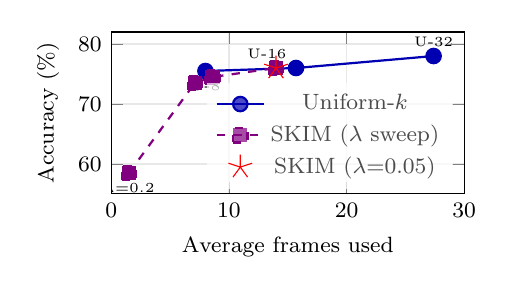
\begin{tikzpicture}
    \begin{axis}[
      width=0.5\linewidth, height=0.3\linewidth,
      xlabel={Average frames used}, ylabel={Accuracy (\%)},
      xmin=0, xmax=30, ymin=55, ymax=82,
      grid=both, grid style={gray!18},
      legend pos=south east,
      legend style={font=\footnotesize, draw=none, fill=white, fill opacity=0.7},
      tick label style={font=\footnotesize}, label style={font=\footnotesize},
      mark size=2.6pt,
    ]
      \addplot[color=blue!70!black, mark=*, thick]
        coordinates {(8.0,75.5) (15.7,76.0) (27.4,78.0)};
      \addlegendentry{Uniform-$k$}
      \addplot[color=violet, mark=square*, thick, dashed]
        coordinates {(1.5,58.5) (7.1,73.5) (8.6,74.5) (14.0,76.0)};
      \addlegendentry{SKIM ($\lambda$ sweep)}
      \addplot[only marks, mark=star, mark size=4.5pt, color=red]
        coordinates {(14.0,76.0)};
      \addlegendentry{SKIM ($\lambda{=}0.05$)}
      \node[font=\tiny, anchor=south] at (axis cs:27.4,78.0) {U-32};
      \node[font=\tiny, anchor=south east] at (axis cs:15.7,76.0) {U-16};
      \node[font=\tiny, anchor=north] at (axis cs:8.0,75.5) {U-8};
      \node[font=\tiny, anchor=north] at (axis cs:1.5,58.5) {$\lambda{=}0.2$};
    \end{axis}
  \end{tikzpicture}
  \caption{Accuracy vs.\ average frames on NExT-QA (val, $n{=}200$). The SKIM
    $\lambda$-sweep traces an accuracy--frame frontier: at $\lambda{=}0.05$ (star) it
    reaches Uniform-16 accuracy ($76.0\%$) using fewer frames, while larger $\lambda$
    spends fewer frames at lower accuracy. SKIM shifts the uniform curve leftward
    (fewer frames at equal accuracy) rather than upward.}
  \label{fig:pareto}
\end{figure}

\section{Analysis}
\label{sec:analysis}

Beyond the headline numbers, we ask \emph{what} the policy learns. Unless noted, this
section uses the $\lambda{=}0.05$ checkpoint on NExT-QA.

\paragraph{The policy adapts its stopping point to the question type.}
Figure~\ref{fig:stopping} shows \emph{where} the policy stops---the position of its
last kept frame---by question type; on average it keeps $14.7$/$13.1$/$13.9$ frames for
causal/temporal/descriptive. The distribution is bimodal (Figure~\ref{fig:retention}),
with one mode at near-immediate stopping and another at running to the forced stop,
but the balance shifts with the question. Descriptive
questions stop earliest (mean last-kept frame at $0.51$ of the video) and causal latest
($0.62$); temporal questions are the most bimodal, with the strongest spike at the final
frame---consistent with needing the whole clip---offset by an early-stop mode that pulls
their mean to $0.55$. The selector is therefore not applying a fixed budget: it spends
frames where the question type warrants it.

\paragraph{When the stop action fires, it fires well.}
Isolating descriptive questions by whether the learned \textsc{stop} action fired is
telling ($n{=}200$ subset). When it does, SKIM answers correctly $93.3\%$ of the time
using only $7.1$ frames; when it never fires and the episode runs to the forced stop,
accuracy falls to $46.2\%$ at $13.0$ frames. Early stopping is thus not the cause of
descriptive errors---if anything, the cases where the policy \emph{cannot} commit to a
stop are the genuinely hard ones it would miss regardless. The aggregate descriptive
number in Table~\ref{tab:nextqa} ($85.7\%$) mixes these two populations.
Figure~\ref{fig:qtype_acc} shows the per-type accuracy breakdown across all methods.

\paragraph{STOP fires less on longer clips (IntentQA transfer).}
The zero-shot transfer to the full IntentQA validation set ($n{=}2{,}044$) reveals
how the stopping behavior adapts to clip length. The policy fires \textsc{stop} early
on $51.7\%$ of IntentQA questions, versus $62.7\%$ on NExT-QA---consistent with
IntentQA videos providing more informative frames per clip. When \textsc{stop} fires,
the policy uses $5.8$ frames at $83.2\%$ accuracy; when the episode runs to the
forced stop, accuracy rises to $90.1\%$ at $26.1$ frames. Unlike the descriptive
split on NExT-QA, running to the end consistently outperforms early stopping on
IntentQA for both causal ($84.4\%$ vs.\ $91.9\%$) and temporal ($79.9\%$ vs.\
$84.9\%$) questions, suggesting the policy has not learned a reliable stopping
criterion for this benchmark's longer, more complex causal chains.

\paragraph{Failure mode: reward hacking via the language prior.}
The cost term that enables a variable budget is also the policy's easiest exploit. As
$\lambda$ grows, stopping early becomes worth more than answering correctly, and at
$\lambda{=}0.2$ the policy degenerates: it keeps $1.5$ frames on average and scores
$58.5\%$ (Table~\ref{tab:nextqa}), close to what the frozen VLM produces from the
question and answer choices alone. In effect the selector learns to stop with almost no
visual evidence and let the VLM answer from its language prior---an exploit made possible
by the well-documented static bias of video-QA benchmarks, where many questions are
answerable from a single frame or none~\citep{atp}. The same pressure appears under
prolonged training at fixed $\lambda$: continuing the $\lambda{=}0.1$ run from $1024$ to
$2528$ episodes shaves the budget from $8.6$ to $7.1$ frames but also trims accuracy
($74.5\%\!\rightarrow\!73.5\%$). Because the reward cannot tell ``answered correctly
\emph{because of} the kept frames'' from ``answered correctly \emph{despite} keeping
almost none,'' $\lambda$ is a brittle knob, and learning a stop criterion reliable across
question types---temporal, not just descriptive---remains the central open problem.

\begin{figure}[t]
  \centering
  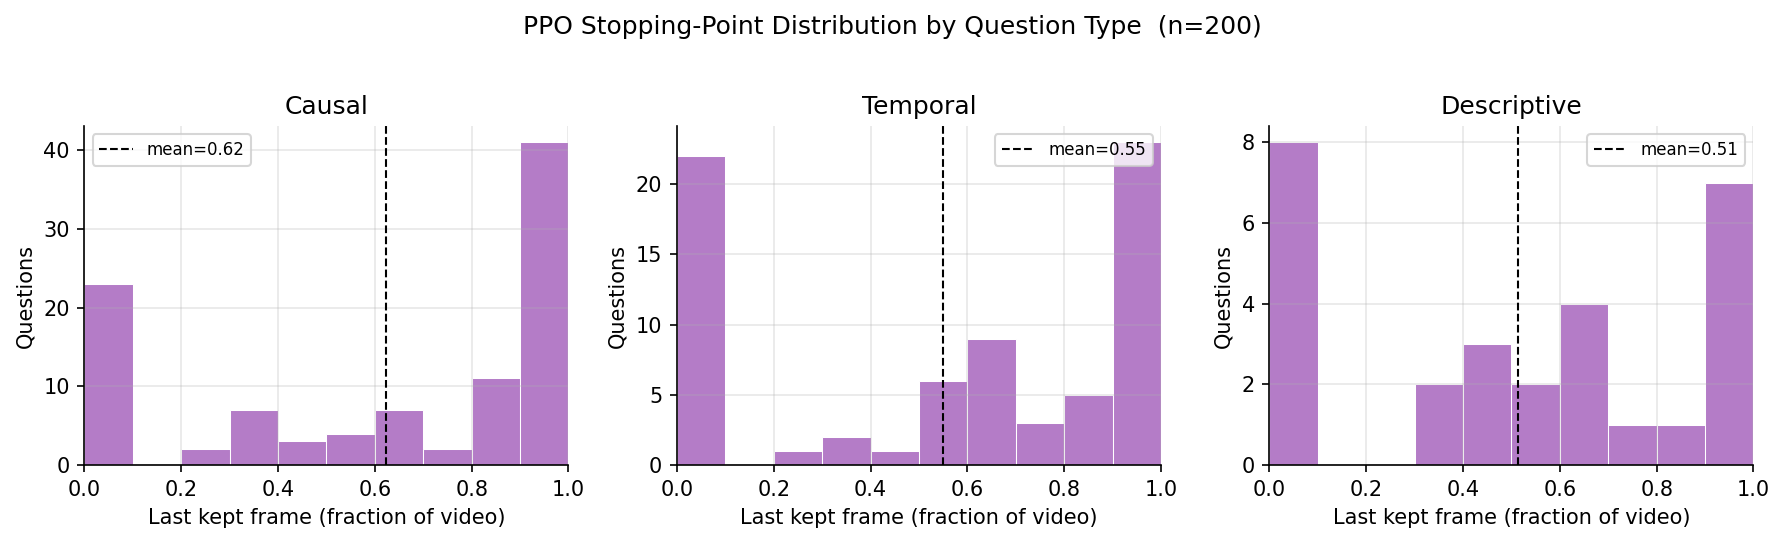
\includegraphics[width=0.72\linewidth]{../results/figures/fig4_stopping_distribution.png}
  \caption{Where SKIM ($\lambda{=}0.05$) stops on NExT-QA, measured as the last kept
    frame's position in the video, by question type. Descriptive questions stop earliest
    (mean $0.51$) and causal latest ($0.62$); temporal shows the strongest mode at the
    final frame (needing the full clip) with an offsetting early-stop mode.}
  \label{fig:stopping}
\end{figure}

\begin{figure}[t]
  \centering
  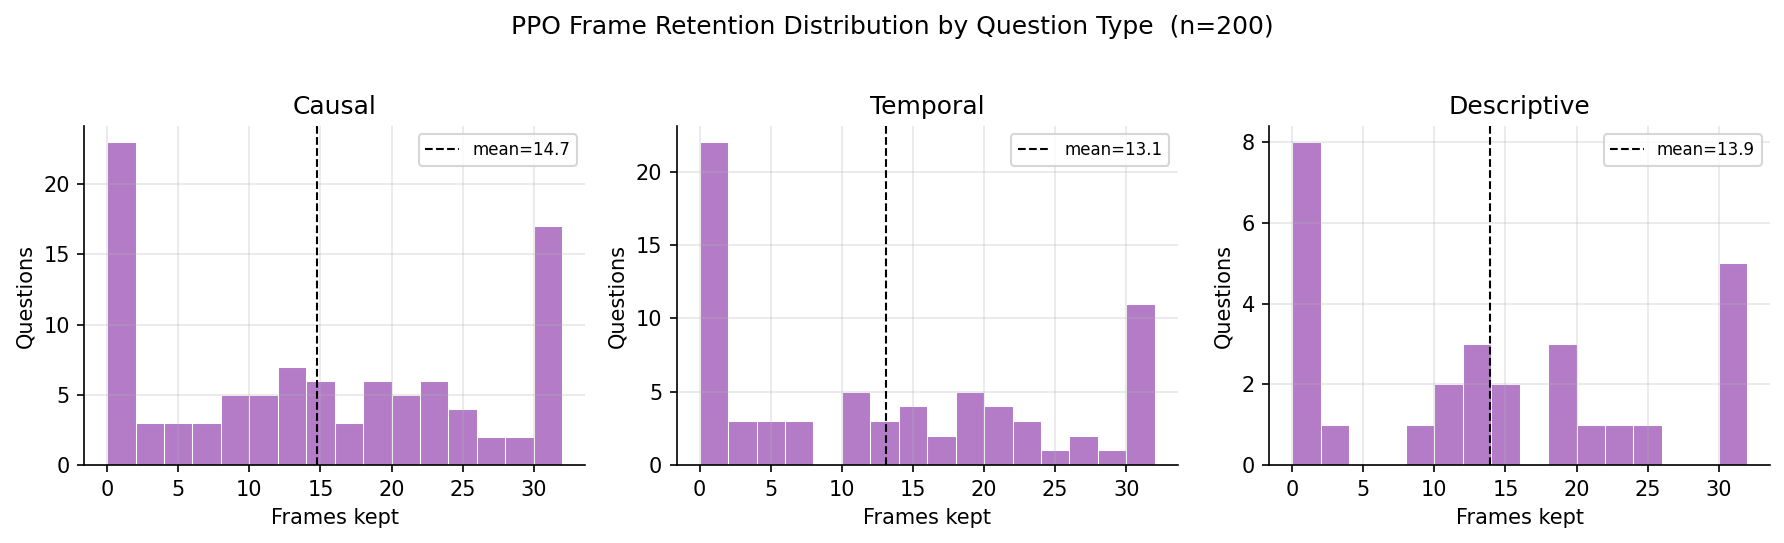
\includegraphics[width=0.72\linewidth]{../results/figures/fig2_retention_by_qtype.png}
  \caption{Distribution of total frames kept by question type (SKIM $\lambda{=}0.05$,
    NExT-QA, $n{=}200$). All three types are bimodal: a large spike near zero (the
    policy fires \textsc{stop} immediately) and a second spike at ${\sim}32$ frames
    (the episode runs to the forced stop). Mean kept frames: causal $14.7$, temporal
    $13.1$, descriptive $13.9$.}
  \label{fig:retention}
\end{figure}

\begin{figure}[t]
  \centering
  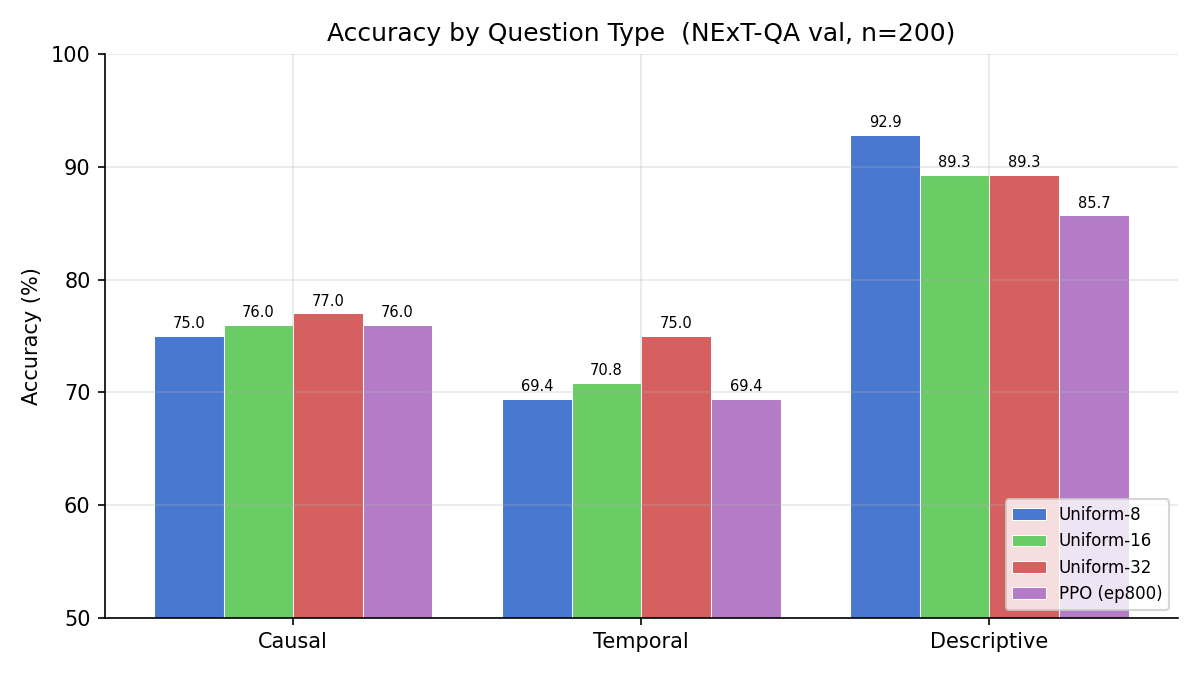
\includegraphics[width=0.72\linewidth]{../results/figures/fig3_accuracy_by_qtype.png}
  \caption{Accuracy by question type on NExT-QA ($n{=}200$) for uniform baselines
    and an intermediate PPO checkpoint (ep800, $\lambda{=}0.1$). Descriptive accuracy
    is highest across all methods but drops for PPO relative to uniform, consistent
    with the early-stopping analysis in this section. Causal accuracy is largely
    unaffected; temporal is most sensitive to frame count.}
  \label{fig:qtype_acc}
\end{figure}

\section{Limitations and Conclusion}
\label{sec:conclusion}

\paragraph{Limitations.}
Our primary ablations use $n{=}200$ validation subsets and a single training run per
setting, so we report point estimates without error bars; relative orderings are
consistent across checkpoints, but small accuracy gaps (e.g., $74.5$ vs.\ $76.0\%$)
should be read as indicative rather than significant. The best SKIM configuration is
validated at $n{=}1{,}000$ on NExT-QA and on the full IntentQA validation set
($n{=}2{,}044$), where results are consistent with the $n{=}200$ ablations. We use a
single frozen backbone (Qwen2.5-VL-3B in 4-bit) on one consumer GPU and have not
tested whether the learned policy transfers across VLM scales or families.
Our IntentQA validation-set accuracy ($86.6\%$) exceeds figures reported in prior
work, but those figures are on the \emph{test} split, not the validation split we use,
making direct comparison unreliable; IntentQA should be read as a zero-shot transfer
test against our own uniform baselines, not a leaderboard comparison.
Most importantly, although SKIM's causal design makes it \emph{compatible} with
streaming, all of our experiments are offline---finite clips capped at $32$ frames
with a forced stop at the end---so we do not evaluate a true streaming deployment,
and we leave EgoSchema evaluation and multi-backbone experiments to future work.

\paragraph{Conclusion.}
SKIM casts adaptive frame selection as a causal, single-pass reinforcement-learning
problem on top of a frozen VLM, trained cheaply on cached embeddings. It matches
uniform sampling at comparable or fewer frames, exposes a controllable accuracy--frame
tradeoff through a single coefficient, and transfers zero-shot across benchmarks. Its
limits are as instructive as its gains: the cost reward that yields a variable budget
is readily hacked via the VLM's language prior, and the policy's stopping behavior is
reliable for some question types but not others. We see the central open problem as
learning a \emph{trustworthy} stop---one that distinguishes having seen enough from
having merely guessed---which is also the prerequisite for the streaming setting this
design is built for. Confidence- or counterfactual-aware rewards, which penalize
answering correctly \emph{without} the kept frames, are a natural next step.

% \begin{ack} ... \end{ack}  % add funding/acknowledgments for the camera-ready (auto-hidden when anonymized)

\bibliographystyle{plainnat}
\bibliography{references}

\appendix
\section{Hyperparameters}
\label{app:hparams}
Table~\ref{tab:hparams} lists all hyperparameters, taken from the configuration files in
\texttt{configs/}. Values are shared across runs except the cost coefficient
$\lambda\in\{0.05,0.1,0.2\}$. Warm-start imitates uniform keep-every-$k$ selection; all
runs use seed $42$ on a single RTX 2070 (8\,GB) and AdamW.

\begin{table}[h]
  \caption{SKIM hyperparameters.}
  \label{tab:hparams}
  \centering
  \begin{tabular}{lll}
    \toprule
    Group & Hyperparameter & Value \\
    \midrule
    Backbone   & model                & Qwen2.5-VL-3B-Instruct \\
               & quantization         & 4-bit NF4 (bfloat16 compute) \\
               & max.\ new tokens     & 16 \\
               & max.\ pixels/frame   & $200{,}704$ ($256\cdot28\cdot28$) \\
    \midrule
    Data       & frame rate           & 1 fps \\
               & max.\ frames $N$     & 32 \\
    \midrule
    Selector   & $d_\text{model}$     & 512 \\
               & layers / heads       & 2 / 4 \\
               & dropout              & 0.1 \\
               & vision / text dim    & 1280 / 2048 \\
               & action dim           & 3 (keep/skip/stop) \\
               & parameters           & ${\approx}8$M \\
    \midrule
    Warm-start & target               & uniform keep-every-$k$ \\
               & epochs / batch       & 3 / 16 \\
               & learning rate        & $1\times10^{-4}$ \\
    \midrule
    PPO        & episodes             & up to 8000 (checkpoints at 1024 / 2528) \\
               & rollout batch        & 32 \\
               & PPO epochs           & 4 \\
               & learning rate        & $3\times10^{-5}$ \\
               & clip range           & 0.2 \\
               & KL coefficient       & 0.05 \\
               & entropy coefficient  & 0.03 \\
               & GAE $\gamma$ / $\lambda_\text{GAE}$ & 1.0 / 0.95 \\
               & cost coeff.\ $\lambda$ & $\{0.05,\,0.1,\,0.2\}$ \\
    \bottomrule
  \end{tabular}
\end{table}

\newpage
\section*{NeurIPS Paper Checklist}

\begin{enumerate}

\item {\bf Claims}
    \item[] Question: Do the main claims made in the abstract and introduction accurately reflect the paper's contributions and scope?
    \item[] Answer: \answerYes{}
    \item[] Justification: The abstract and Section~\ref{sec:intro} state the contributions and scope, including the explicit caveat that SKIM matches but does not exceed the uniform accuracy--frame frontier.

\item {\bf Limitations}
    \item[] Question: Does the paper discuss the limitations of the work performed by the authors?
    \item[] Answer: \answerYes{}
    \item[] Justification: Section~\ref{sec:conclusion} discusses the $n{=}200$ subsets and lack of error bars, the single 3B backbone, offline-only evaluation (streaming is a design property, not measured), and the unsolved reward-hacking failure.

\item {\bf Theory assumptions and proofs}
    \item[] Question: For each theoretical result, does the paper provide the full set of assumptions and a complete (and correct) proof?
    \item[] Answer: \answerNA{}
    \item[] Justification: The paper makes no theoretical claims.

\item {\bf Experimental result reproducibility}
    \item[] Question: Does the paper fully disclose all the information needed to reproduce the main experimental results of the paper to the extent that it affects the main claims and/or conclusions of the paper (regardless of whether the code and data are provided or not)?
    \item[] Answer: \answerYes{}
    \item[] Justification: Sections~\ref{sec:method}--\ref{sec:experiments} specify the MDP, policy architecture, training procedure, datasets, and evaluation protocol; Appendix~\ref{app:hparams} lists all hyperparameters.

\item {\bf Open access to data and code}
    \item[] Question: Does the paper provide open access to the data and code, with sufficient instructions to faithfully reproduce the main experimental results, as described in supplemental material?
    \item[] Answer: \answerYes{}
    \item[] Justification: Code, configuration files, evaluation scripts, and result JSONs are publicly available at \url{https://github.com/IshanKat/skim}. The datasets (NExT-QA, IntentQA) are publicly available from their respective authors.

\item {\bf Experimental setting/details}
    \item[] Question: Does the paper specify all the training and test details (e.g., data splits, hyperparameters, how they were chosen, type of optimizer) necessary to understand the results?
    \item[] Answer: \answerYes{}
    \item[] Justification: Section~\ref{sec:experiments} gives datasets, splits, baselines, and metrics; Appendix~\ref{app:hparams} gives the optimizer and all hyperparameters.

\item {\bf Experiment statistical significance}
    \item[] Question: Does the paper report error bars suitably and correctly defined or other appropriate information about the statistical significance of the experiments?
    \item[] Answer: \answerNo{}
    \item[] Justification: Results use $n{=}200$ subsets and a single training run per setting without error bars; this is stated as a limitation in Section~\ref{sec:conclusion}, and small accuracy gaps are described as indicative.

\item {\bf Experiments compute resources}
    \item[] Question: For each experiment, does the paper provide sufficient information on the computer resources (type of compute workers, memory, time of execution) needed to reproduce the experiments?
    \item[] Answer: \answerYes{}
    \item[] Justification: Section~\ref{sec:experiments} reports a single RTX 2070 (8\,GB); the design uses exactly one VLM forward pass per episode, on pre-cached embeddings.

\item {\bf Code of ethics}
    \item[] Question: Does the research conducted in the paper conform, in every respect, with the NeurIPS Code of Ethics \url{https://neurips.cc/public/EthicsGuidelines}?
    \item[] Answer: \answerYes{}
    \item[] Justification: The research uses public benchmarks and a publicly available model and conforms to the NeurIPS Code of Ethics.

\item {\bf Broader impacts}
    \item[] Question: Does the paper discuss both potential positive societal impacts and negative societal impacts of the work performed?
    \item[] Answer: \answerNA{}
    \item[] Justification: The work improves the efficiency of video question answering; it has no direct societal impact beyond those common to the underlying VLM.

\item {\bf Safeguards}
    \item[] Question: Does the paper describe safeguards that have been put in place for responsible release of data or models that have a high risk for misuse (e.g., pre-trained language models, image generators, or scraped datasets)?
    \item[] Answer: \answerNA{}
    \item[] Justification: The paper releases no data or models with a high risk of misuse.

\item {\bf Licenses for existing assets}
    \item[] Question: Are the creators or original owners of assets (e.g., code, data, models), used in the paper, properly credited and are the license and terms of use explicitly mentioned and properly respected?
    \item[] Answer: \answerYes{}
    \item[] Justification: We cite and use Qwen2.5-VL~\citep{qwen25vl}, NExT-QA~\citep{nextqa}, and IntentQA~\citep{intentqa} under their respective licenses and terms of use.

\item {\bf New assets}
    \item[] Question: Are new assets introduced in the paper well documented and is the documentation provided alongside the assets?
    \item[] Answer: \answerNA{}
    \item[] Justification: The paper does not release new datasets or models.

\item {\bf Crowdsourcing and research with human subjects}
    \item[] Question: For crowdsourcing experiments and research with human subjects, does the paper include the full text of instructions given to participants and screenshots, if applicable, as well as details about compensation (if any)?
    \item[] Answer: \answerNA{}
    \item[] Justification: The paper involves no crowdsourcing or research with human subjects.

\item {\bf Institutional review board (IRB) approvals or equivalent for research with human subjects}
    \item[] Question: Does the paper describe potential risks incurred by study participants, whether such risks were disclosed to the subjects, and whether Institutional Review Board (IRB) approvals (or an equivalent approval/review based on the requirements of your country or institution) were obtained?
    \item[] Answer: \answerNA{}
    \item[] Justification: The paper involves no human-subjects research.

\item {\bf Declaration of LLM usage}
    \item[] Question: Does the paper describe the usage of LLMs if it is an important, original, or non-standard component of the core methods in this research? Note that if the LLM is used only for writing, editing, or formatting purposes and does \emph{not} impact the core methodology, scientific rigor, or originality of the research, declaration is not required.
    \item[] Answer: \answerYes{}
    \item[] Justification: A frozen vision--language model (Qwen2.5-VL-3B) is integral to the method---as both the reward signal and the answerer---and is described in Section~\ref{sec:method}.

\end{enumerate}


\end{document}
